\documentclass{beamer}

\newcommand{\cmd}[1]{\textbf{\texttt{#1}}}
\newcommand{\pkg}[1]{\texttt{#1}}
\newcommand{\env}[1]{\texttt{#1}}
\newcommand{\opt}[1]{\textsl{#1}}

\usepackage{beamerthemesplit}
\beamertemplatenavigationsymbolsempty
\setbeamertemplate{footline}[page number]{}

\usepackage{graphicx}
\usepackage{color}
\usepackage{listings}
\usepackage{verbatim}
\usepackage{setspace}
\usepackage{url}

\usepackage{fontspec}
\setmonofont{Latin Modern Mono}
\setsansfont{TeX Gyre Heros}

\lstset{breakatwhitespace=true,
language=C++,
basicstyle=\footnotesize\ttfamily,
keywordstyle=\color{blue}\ttfamily,
stringstyle=\color{red}\ttfamily,
commentstyle=\color{brown}\ttfamily,
morecomment=[l][\color{magenta}]{\#}keepspaces=true,
breaklines=true,
tabsize=3,
showstringspaces=false,
extendedchars=true,
frame=single}

\newcommand*{\vcenteredhbox}[1]{\begingroup
\setbox0=\hbox{#1}\parbox{\wd0}{\box0}\endgroup}

\usepackage{tikz}
\usetikzlibrary{matrix}
\usepackage{ragged2e}

\tikzstyle{component} = [rectangle, rounded corners, minimum width=5cm, text width=4cm, minimum height=0.8cm,text centered, draw=black, fill=red!30]
\tikzstyle{repo} = [rectangle, minimum width=5cm, text width=4cm, minimum height=0.8cm, text centered, draw=black, fill=orange!30]
\tikzstyle{newrepo} = [rectangle, minimum width=5cm, text width=4cm, minimum height=0.8cm, text centered, draw=black, fill=orange!60]

\tikzstyle{arrow} = [thick,->,>=stealth]
\tikzstyle{darrow} = [thick,<->,>=stealth]

\newcommand*{\abox}[1]{\framebox{\hbox to 0.5cm{\texttt\{{\\hss#1\hss}}}}

\title{C++ status}
\author{Roger Leigh}
\date{May 2017}

\begin{document}

\begin{frame}[plain,fragile]
  \titlepage

  \begin{center}
    \textsl{Progress over the last year and upcoming features}
  \end{center}
\end{frame}

\begin{frame}[fragile]
  \frametitle{Component splitting: completed}
  \begin{center}
    \begin{tikzpicture}[y=-1cm]
      \onslide<1->{
        \node (bfrepo) [repo] {bioformats.git};
        \node (c1) [component, below of=bfrepo, yshift=-0.3cm] {ome-compat};
        \node (c2) [component, below of=c1, yshift=-0.3cm] {ome-common};
        \node (c3) [component, below of=c2, yshift=-0.3cm] {ome-xml};
        \node (c4) [component, below of=c3, yshift=-0.3cm] {ome-bioformats};
        \node (c5) [component, below of=c4, yshift=-0.3cm] {ome-qtwidgets};

        \draw [thick] (bfrepo.south) -- (c1.north);
        \draw [thick] (c1.south) -- (c2.north);
        \draw [thick] (c2.south) -- (c3.north);
        \draw [thick] (c3.south) -- (c4.north);
        \draw [thick] (c4.south) -- (c5.north);
      }
      \onslide<2->{
        \node (sb) [repo, right of=bfrepo, xshift=5cm] {ome-cmake-superbuild.git};
        \node (commonrepo) [repo, right of=c2, xshift=5cm, yshift=0.7cm] {ome-common-cpp.git};
        \node (xmlrepo) [newrepo, right of=c3, xshift=5cm] {ome-model.git};
        \node (filesrepo) [repo, right of=c4, xshift=5cm] {ome-files-cpp.git};
        \node (qtrepo) [repo, right of=c5, xshift=5cm] {ome-qtwidgets.git};

        \draw [arrow] (bfrepo) -- (sb);
        \draw [arrow] (c1) -- (commonrepo);
        \draw [arrow] (c2) -- (commonrepo);
        \draw [arrow] (c3) -- (xmlrepo);
        \draw [arrow] (c4) -- (filesrepo);
        \draw [arrow] (c5) -- (qtrepo);
      }
    \end{tikzpicture}
  \end{center}
\end{frame}

\begin{frame}[fragile]
  \frametitle{Major changes: Windows support}

  \begin{itemize}
  \item Added support for VS2015
  \item Dropped support for VS2012
  \item Added command line tools
  \item Numerous fixes and enhancements
    \pause
  \item DLLs not yet supported
  \end{itemize}
\end{frame}

\begin{frame}[fragile]
  \frametitle{Major changes: data model}

  \begin{itemize}
  \item Added 2015-01 model support
  \item Added 2016-06 model support
    \pause
  \item BinData
  \item Units
  \item Map annotations
  \item ROI transforms
  \end{itemize}
\end{frame}

\begin{frame}[fragile]
  \frametitle{Major changes: TIFF readers and writers}

  \begin{itemize}
  \item Performance testing
  \item added default strip size heuristic
  \item added OME-TIFF validity checks, metadata caching, file caching, plane element handling
  \item added TIFF compression
  \item fixed interleaving (PlanarConfiguration) behaviour
  \item added IFD offset caching
  \end{itemize}

  \begin{lstlisting}[language=C++]
    writer.setCompression("lzw");
    writer.setInterleaved(false);
    writer.setTileSizeX(512U);
    writer.setTileSizeY(512U);
  \end{lstlisting}
\end{frame}

\begin{frame}[fragile]
  \frametitle{Major changes: other}

  \begin{itemize}
  \item Native unit and quantity support
  \item C++11/14
  \item Updated examples
  \end{itemize}
  \pause

  \begin{lstlisting}[language=C++]
    typedef model::primitives::Quantity
      <model::enums::UnitsLength,
       model::primitives::PositiveFloat> PositiveLength;
    metadatastore.setPixelsPhysicalSizeX
      (PositiveLength(118.2, model::enums::UnitsLength::MICROMETER), 0);

    // C++11
    metadatastore.setPixelsPhysicalSizeX
      ({118.2, UnitsLength::MICROMETER}, 0);

    //  Low level Boost.Units
    micrometre_quantity len(118.2);
  \end{lstlisting}
\end{frame}

\begin{frame}[fragile]
  \frametitle{Performance testing}
  \begin{centering}
    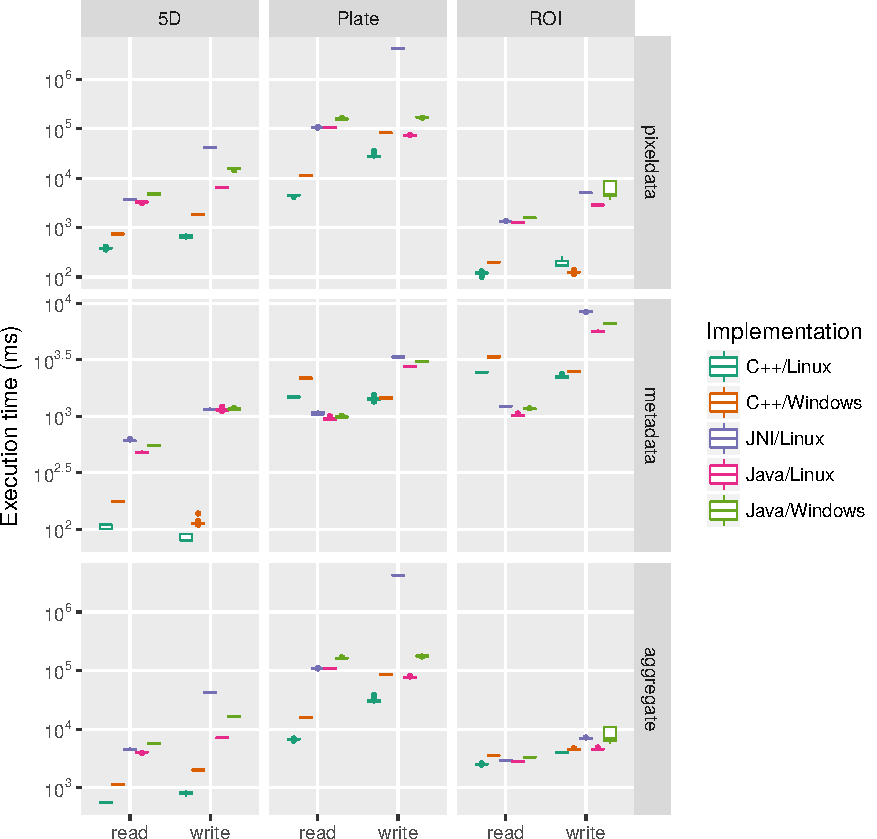
\includegraphics[width=0.8\textwidth]{cpp-dundee-2017-figures/files-suppfig5}
  \end{centering}
\end{frame}

\begin{frame}[fragile]
  \frametitle{Performance testing}
  \begin{centering}
    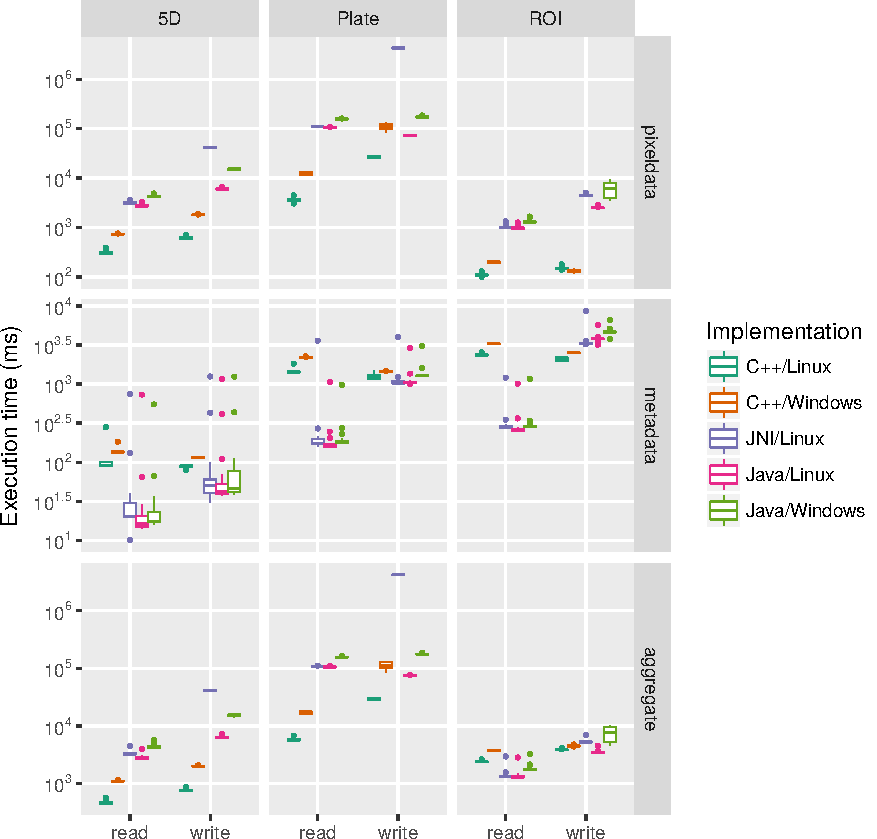
\includegraphics[width=0.8\textwidth]{cpp-dundee-2017-figures/files-suppfig6}
  \end{centering}
\end{frame}

\begin{frame}[fragile]
  \frametitle{Python API}

  \begin{itemize}
  \item \url{https://github.com/ome/ome-files-py}
  \item Core: Python extension module that wraps the C++ API
  \item Can open image planes as NumPy arrays
  \item Work in progress: exposes a subset of \texttt{OMETIFFReader}
  \end{itemize}
  \begin{columns}
    \begin{column}{0.05\textwidth}
    \end{column}
    \begin{column}{0.65\textwidth}
      \centering
      \begin{lstlisting}[language=Python]
import ome_files
import matplotlib.pyplot as plt

reader = ome_files.OMETIFFReader()
reader.set_id("tubhiswt_C0.ome.tif")
pixels = reader.open_array(0)
reader.close()
plt.imshow(pixels, cmap="gray")
plt.show()
      \end{lstlisting}
    \end{column}
    \begin{column}{0.4\textwidth}
      \centering
      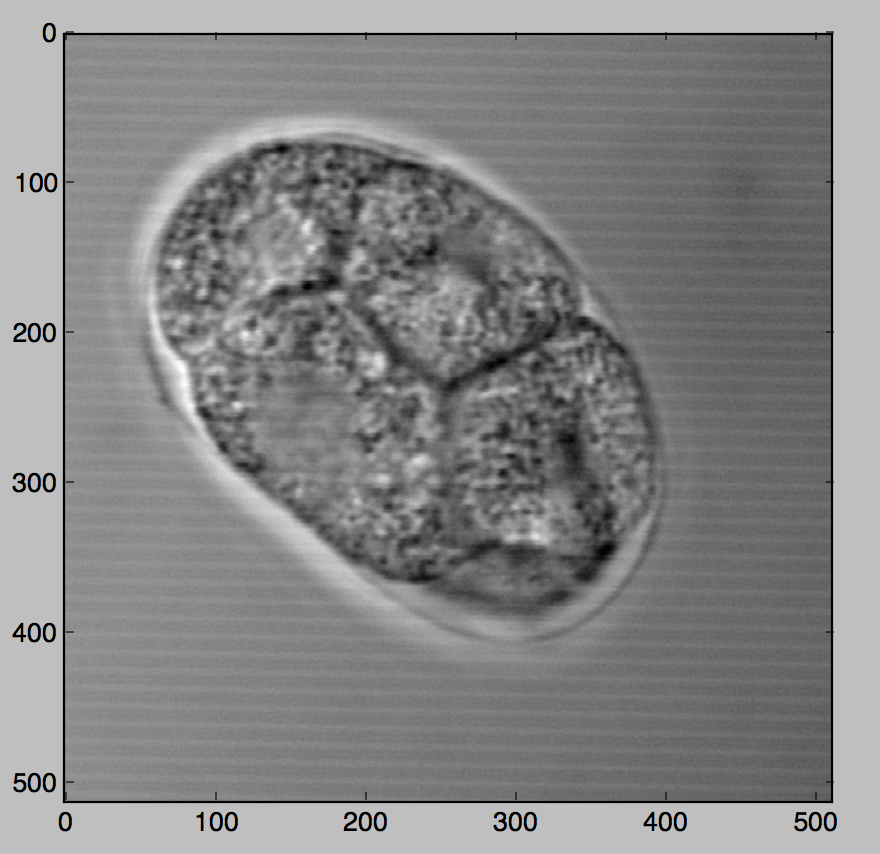
\includegraphics[width=0.85\textwidth]{cpp-dundee-2017-figures/openbytes.png}
    \end{column}
  \end{columns}
\end{frame}

\begin{frame}[fragile]
  \frametitle{Upcoming changes (0.4.x)}

  \begin{itemize}
  \item Add support for VS2017
  \item Drop support for VS2013 (deprecate, EOL)
  \item Flexible model API
  \item Options API (YAML?)
  \end{itemize}
\end{frame}

\begin{frame}[fragile]
  \frametitle{Future thoughts}

  \begin{itemize}
  \item API cleanup
  \item Modulo support
  \item HDF5
  \item Windows DLLs
  \item nD pixel buffer
  \end{itemize}
\end{frame}

\end{document}
